\documentclass{standalone}
\usepackage{tikz}
\usepackage{xcolor}
\usetikzlibrary{patterns, positioning}
\usetikzlibrary{shapes.misc}
\usepackage[outline]{contour}
\contourlength{1.5pt} 

    \usetikzlibrary{calc}
    \usepackage{relsize}
    \tikzset{fontscale/.style = {font=\relsize{#1}}}
\newsavebox{\myboxRACA} 
\begin{lrbox}{\myboxRACA}
  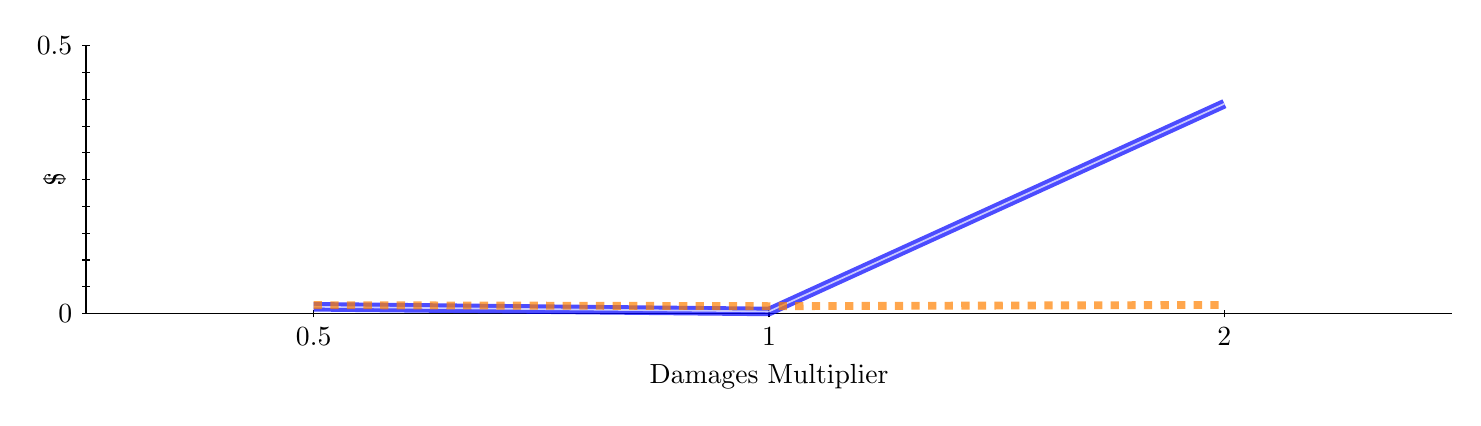
\begin{tikzpicture}
    \begin{scope}
% 
% Cell 0,0
% 
\draw[black] (0.8,1.1) -- (0.8,4.5);
\node[rotate=90, fontscale=0.7, anchor=center] at (0.4, 2.8) {\$};
\draw[black] (0.75,1.1) -- (0.85,1.1);
\node[fontscale=0.7, anchor=east] at (0.75, 1.1) {0};
\draw[black] (0.75,1.44) -- (0.85,1.44);
\node[fontscale=0.7, anchor=east] at (0.75, 1.44) { };
\draw[black] (0.75,1.78) -- (0.85,1.78);
\node[fontscale=0.7, anchor=east] at (0.75, 1.78) { };
\draw[black] (0.75,2.12) -- (0.85,2.12);
\node[fontscale=0.7, anchor=east] at (0.75, 2.12) { };
\draw[black] (0.75,2.46) -- (0.85,2.46);
\node[fontscale=0.7, anchor=east] at (0.75, 2.46) { };
\draw[black] (0.75,2.8) -- (0.85,2.8);
\node[fontscale=0.7, anchor=east] at (0.75, 2.8) { };
\draw[black] (0.75,3.14) -- (0.85,3.14);
\node[fontscale=0.7, anchor=east] at (0.75, 3.14) { };
\draw[black] (0.75,3.48) -- (0.85,3.48);
\node[fontscale=0.7, anchor=east] at (0.75, 3.48) { };
\draw[black] (0.75,3.82) -- (0.85,3.82);
\node[fontscale=0.7, anchor=east] at (0.75, 3.82) { };
\draw[black] (0.75,4.16) -- (0.85,4.16);
\node[fontscale=0.7, anchor=east] at (0.75, 4.16) { };
\draw[black] (0.75,4.5) -- (0.85,4.5);
\node[fontscale=0.7, anchor=east] at (0.75, 4.5) {$0.5$};

\draw[black] (0.8,1.1) -- (18.15,1.1);
\node[fontscale=0.7, anchor=center] at (9.475, 0.3) {Damages Multiplier};
\draw[black] (3.6917,1.05) -- (3.6917,1.15);
\node[fontscale=0.7, anchor=north] at (3.6917, 1.05) {0.5};
\draw[black] (9.475,1.05) -- (9.475,1.15);
\node[fontscale=0.7, anchor=north] at (9.475, 1.05) {1};
\draw[black] (15.258,1.05) -- (15.258,1.15);
\node[fontscale=0.7, anchor=north] at (15.258, 1.05) {2};

\draw[blue, opacity=0.70, line width=0.5mm, double] (3.6917,1.1854) -- (9.475,1.1263) -- (15.258,3.7645);
\draw[orange, opacity=0.70, line width=1mm, dashed] (3.6917,1.2063) -- (9.475,1.1932) -- (15.258,1.2092);

  \end{scope}
  \end{tikzpicture}
\end{lrbox}

\begin{document}
\begin{tikzpicture}
\clip(0, -1) rectangle + (20,7.3); 
\draw[black] (1.7,1.5) -- (1.7,6.3);
\node[rotate=90, fontscale=2, anchor=center] at (0.7, 4.45) {Costs Multiplier};
\draw[black] (1.65,4.45) -- (1.75,4.45);
\node[fontscale=2, anchor=east] at (1.65, 4.45) {1};

\draw[black] (1.7,1.5) -- (20,1.5);
\node[fontscale=2, anchor=center] at (11.25, 0.6) {};
\draw[black] (11.25,1.45) -- (11.25,1.55);
\node[fontscale=2, anchor=north] at (11.25, 1.45) {Baseline Values};


\node[anchor=north west,inner sep=0pt,outer sep=0pt] at (1.75,6.2) { \usebox{\myboxRACA} };
\draw (11.25,0) node[draw=none] (baseCoordinate) {};
\begin{scope}[align=center]
        \matrix[scale=0.5, draw=black, below=-0.4cm of baseCoordinate, nodes={draw}, column sep=0.1cm]{
        
\draw[blue, opacity=0.70, line width=0.5mm, double] (0.25,-0.25) -- (0.75,-0.25); &
\node[draw=none, font=\small] (B) {False Positive Inaccuracy}; &

\draw[orange, opacity=0.70, line width=1mm, dashed] (0.25,-0.25) -- (0.75,-0.25); &
\node[draw=none, font=\small] (B) {False Negative Inaccuracy}; \\
            };
\end{scope}

\end{tikzpicture}
\end{document}